\documentclass{standalone}
\usepackage{tikz}
\usetikzlibrary{arrows.meta}
\begin{document}
   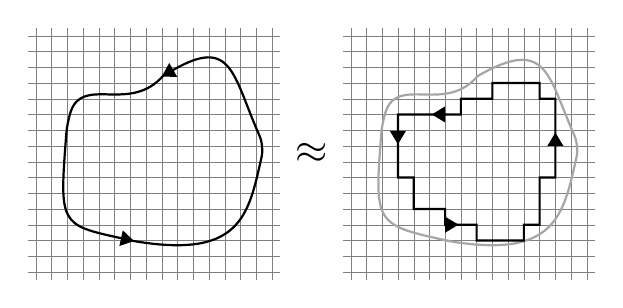
\begin{tikzpicture}[thick]
    
       \draw[line width=0.1pt,draw=black!50,step=0.2] (-0.1,-0.1) grid (3.1,3.1);
     
     
       \draw[rounded corners,-Triangle] (1.2,0.4)..controls(2.6,0.15)and(2.7,0.7) ..(2.9,1.6) ..controls(2.5,2.5)and(2.5,3)..(1.6,2.48);
       \draw[rounded corners,-Triangle] (1.627,2.5)..controls(1.2,2)and(0.6,2.5) ..(0.4,1.9)..controls(0.3,0.6) ..(1.25,0.392);
        \node[scale=1.5] at (3.5,1.5) {$\approx$};

        \begin{scope}[xshift=4cm]
            \draw[line width=0.1pt,draw=black!50,step=0.2] (-0.1,-0.1) grid (3.1,3.1);
            \draw[gray!70,rounded corners] (1.2,0.4)..controls(2.6,0.15)and(2.7,0.7) ..(2.9,1.6) ..controls(2.5,2.5)and(2.5,3)..(1.6,2.48);
            \draw[gray!70,rounded corners] (1.615,2.49)..controls(1.2,2)and(0.6,2.5) ..(0.4,1.9)..controls(0.3,0.6) ..(1.25,0.392);

            \draw[] (0.6,2)--++(0,-0.8)--++(0.2,0)--++(0,-0.4)--++(0.4,0)--++(0,-0.2)--++(0.4,0)--++(0,-0.2)--++(0.6,0)--++(0,0.2)
            --++(0.2,0)--++(0,0.6)--++(0.2,0)--++(0,1)--++(-0.2,0)--++(0,0.2)--++(-0.6,0)--++(0,-0.2)--++(-0.4,0)--++(0,-0.2)--cycle;

            \draw[-Triangle] (0.6,2)--++(0,-0.38);
            \draw[-Triangle] (1.2,0.6)--++(0.17,0);
            \draw[-Triangle] (2.6,1.6)--++(0,0.17);
            \draw[-Triangle] (1.2,2)--++(-0.17,0);
        \end{scope}
   
    \end{tikzpicture}
\end{document}